\documentclass[11pt]{article}

\usepackage{latexsym}
\usepackage{amssymb}
\usepackage{amsthm}
\usepackage{enumerate}
\usepackage{amsmath}
\usepackage{graphicx}
\usepackage{cancel}
\numberwithin{equation}{section}

\setlength{\evensidemargin}{.25in}
\setlength{\oddsidemargin}{-.25in}
\setlength{\topmargin}{-.75in}
\setlength{\textwidth}{6.5in}
\setlength{\textheight}{9.5in}
\newcommand{\due}{September 9th, 2015}
\newcommand{\HWnum}{1}
\newcommand{\grad}{\bold\nabla}
\newcommand{\vecE}{\vec{E}}
\newcommand{\scrptR}{\vec{\mathfrak{R}}}
\newcommand{\kapa}{\frac{1}{4\pi\epsilon_0}}
\newcommand{\emf}{\mathcal{E}}
\newcommand{\unit}[1]{\ensuremath{\, \mathrm{#1}}}
\newcommand{\real}{\textnormal{Re}}
\newcommand{\Erf}{\textnormal{Erf}}
\newcommand{\sech}{\textnormal{sech}}
\newcommand{\scrO}{\mathcal{O}}
\newcommand{\levi}{\widetilde{\epsilon}}
\newcommand{\partiald}[2]{\ensuremath{\frac{\partial{#1}}{\partial{#2}}}}
\newcommand{\norm}[2]{\langle{#1}|{#2}\rangle}
\newcommand{\inprod}[2]{\langle{#1}|{#2}\rangle}
\newcommand{\ket}[1]{|{#1}\rangle}
\newcommand{\bra}[1]{\langle{#1}|}





\begin{document}
\begin{titlepage}
\setlength{\topmargin}{1.5in}
\begin{center}
\Huge{Physics 3320} \\
\LARGE{Principles of Electricity and Magnetism II} \\
\Large{Professor Ana Maria Rey} \\[1cm]

\huge{Homework \#\HWnum}\\[0.5cm]

\large{Joe Becker} \\
\large{SID: 810-07-1484} \\
\large{\due} 

\end{center}

\end{titlepage}



\section{Problem \#1}
We note that for a given force, $\mathbf{F}$, we can say that $\mathbf{F}$ has an associated
potential energy if the force is a \emph{conservative force}. We can test if a force is 
conservative if a closed path integral over $\mathbf{F}$ is \emph{path independent} which 
implies that
\begin{equation}
\oint\mathbf{F}\cdot d\mathbf{r} = 0\textnormal{.}
\label{PathInd}
\end{equation}
Now if we apply \emph{Stoke's Theorem} we find that equation \ref{PathInd} becomes
$$\int_{A}(\grad\times\mathbf{F})\cdot d\mathbf{a} = 0\textnormal{.}$$
which implies that
\begin{equation}
\grad\times\mathbf{F} = 0.
\label{ConTest}
\end{equation}
We note that equation \ref{ConTest} implies that there exists a scaler function that is 
given by 
\begin{equation}
\mathbf{F} = -\grad V(\mathbf{r})
\label{PotEn}
\end{equation}
where $V(\mathbf{r})$ is called the \emph{Potential Energy}.
So, we can use equation \ref{ConTest} to test if a given force is conservative and then use
equation \ref{PotEn} to find it's associated potential energy.

\begin{enumerate}[(a)]
\item Given that $F_x = ay$, $F_y=F_z=0$ we can test if if equation \ref{ConTest} holds 
true for the force 
$$\mathbf{F} = \left(\begin{array}{c}
                        ay\\
                        0\\
                        0\\
            \end{array}\right)$$
by
\begin{align*}
\grad\times\mathbf{F} &= \det\left|\begin{array}{ccc} \hat{x}     &\hat{y}     &\hat{z}\\
                                                   \partial_x  &\partial_y  &\partial_z\\
                                                   ay          &0           &0
                          \end{array}\right|\\
&= 0\hat{x} + \cancelto{0}{\partial_z(ay)\hat{y}} - \partial_y(ay)\hat{z}\\
&= -a\hat{z}\ne 0
\end{align*}
So, we can see that $\mathbf{F}$ is a not conservative force. Therefore there does not exist 
a potential energy associated with this force.


\item Given the force
$$\mathbf{F} = a\frac{\mathbf{r}}{r^3}$$
where $r = \sqrt{x^2+y^2+z^2}$ and $\mathbf{r} = (x,y,z)$. We test if equation \ref{ConTest} is true by first noting that this equation is spherically symmetric so we choose to work in spherical coordinates 
and that the unit vector $\hat{r}$ is given by
$$\hat{r} = \frac{\mathbf{r}}{r}$$
which implies that our force can be written as
$$\mathbf{F} = a\frac{1}{r^2}\frac{\mathbf{r}}{r} = a\frac{\hat{r}}{r^2}.$$
Now we are able to solve equation \ref{ConTest} in spherical coordinates by
\begin{align*}
\grad\times\mathbf{F} &= \det\left|\begin{array}{ccc} 
       \hat{r}       &\hat{\theta}                   &\hat{\phi}\\
       \partial_r    &\dfrac{1}{r}\partial_{\theta}  &\dfrac{1}{r\sin(\theta)}\partial_{\phi}\\
       \dfrac{a}{r^2} &0                             &0
                          \end{array}\right|\\
&= 0\hat{r} + \frac{1}{r\sin(\theta)}\cancelto{0}{\partial_{\phi}\left(\frac{a}{r^2}\right)}\hat{\theta} + \frac{1}{r}\cancelto{0}{\partial_{\theta}\left(\frac{a}{r^2}\right)}\hat{\phi}\\
&= 0
\end{align*}
So we see that equation \ref{ConTest} holds true. Therefore we can find the associated 
potential energy to $\mathbf{F}$ by solving equation \ref{PotEn} for $V(\mathbf{r})$. 
\begin{align*}
\mathbf{F}(\mathbf{r}) &= -\grad V(\mathbf{r})\\
&\Downarrow\\
V(\mathbf{r}) &= -\int_{0}^{\mathbf{r}}\mathbf{F}(\mathbf{r'})\cdot d\mathbf{r'}
\end{align*}
Note in spherical coordinates our differential becomes
$$d\mathbf{r} = dr\hat{r} + rd\theta\hat{\theta} + r\sin(\theta)d\phi\hat{\phi}.$$
So we can solve for $\mathbf{F}(\mathbf{r})$ by
\begin{align*}
V(\mathbf{r}) &= -\int_{0}^{\mathbf{r}}\mathbf{F}(\mathbf{r'})\cdot d\mathbf{r'}\\
&= -\int_{0}^{\mathbf{r}}\left(a\frac{\hat{r'}}{r'^2}\right)\cdot\left(dr'\hat{r} + r'd\theta'\hat{\theta} + r'\sin(\theta')d\phi'\hat{\phi}\right)\\
&= -\int_{0}^{r}\frac{a}{r'^2}dr' \\
&= -a\left(\frac{1}{r'}\right|^{r} \\
&\Downarrow\\
V(r) &= a\frac{1}{r}
\end{align*}

\item Given that $F_x = a\frac{y}{r}$, $F_y=-a\frac{x}{r^2}$, and $F_z=0$ we can test if if 
equation \ref{ConTest} holds true for the force 
$$\mathbf{F} = \left(\begin{array}{c}
                        a\dfrac{y}{r}\\
                        -a\dfrac{x}{r^2}\\
                        0
            \end{array}\right)
= \left(\begin{array}{c}
                        a\dfrac{r\sin(\theta)\cos(\phi)}{r}\\
                        -a\dfrac{r\sin(\theta)\sin(\phi)}{r^2}\\
                        0
  \end{array}\right)
= \left(\begin{array}{c}
                        a{\sin(\theta)\cos(\phi)}\\
                        -a\dfrac{\sin(\theta)\sin(\phi)}{r}\\
                        0
  \end{array}\right)$$
Note that we converted $x$ and $y$ to spherical coordinates. Again we use equation 
\ref{ConTest} to see if this force is conservative.
\begin{align*}
\grad\times\mathbf{F} &= \det\left|\begin{array}{ccc} 
 \hat{r}                    &\hat{\theta}                        &\hat{\phi}\\
 \partial_r                 &\dfrac{1}{r}\partial_{\theta}       &\dfrac{1}{r\sin(\theta)}\partial_{\phi}\\
 a{\sin(\theta)\cos(\phi)}  &-a\dfrac{\sin(\theta)\sin(\phi)}{r} &0
                          \end{array}\right|\\
&= -\frac{1}{r\cancel{\sin(\theta)}}\partial_{\phi}\left(-a\frac{\cancel{\sin(\theta)}\sin(\phi)}{r}\right)\hat{r}\\
& \ \ \ \ \ + \frac{1}{r\cancel{\sin(\theta)}}\partial_{\phi}\left(a{\cancel{\sin(\theta)}\cos(\phi)}\right)\hat{\theta}\\ 
& \ \ \ \ \ + \left(\partial_{r}\left(-a\dfrac{\sin(\theta)\sin(\phi)}{r}\right) - \frac{1}{r}\partial_{\theta}\left(a\sin(\theta)\cos(\phi)\right)\right)\hat{\phi}\\
&= -\frac{a\cos(\phi)}{r^2}\hat{r} - \frac{a\sin(\phi)}{r}\hat{\theta} 
   + \left(a\dfrac{\sin(\theta)\sin(\phi)}{r^2} 
   - \frac{a\cos(\theta)\cos(\phi)}{r}\right)\hat{\phi} \ne 0
\end{align*}
Therefore the force that is given is not a conservative force. This implies that there does
not exist a potential energy for said force.
\end{enumerate}
\pagebreak

\section{Problem \#2}
\begin{enumerate}[(a)]

\item Given the potential energy $V(x) = A|x|^n$ where $A>0$ and $n=1,2,3,...$ we can plot
the potential as shown in Figure \ref{Prob2a}. Note that the dotted line designates the 
energies that have bounded oscillations. As we see in figure \ref{Prob2a} that the energy 
range for bounded oscillations is
$$0<E<\infty.$$
\begin{figure}
\centering
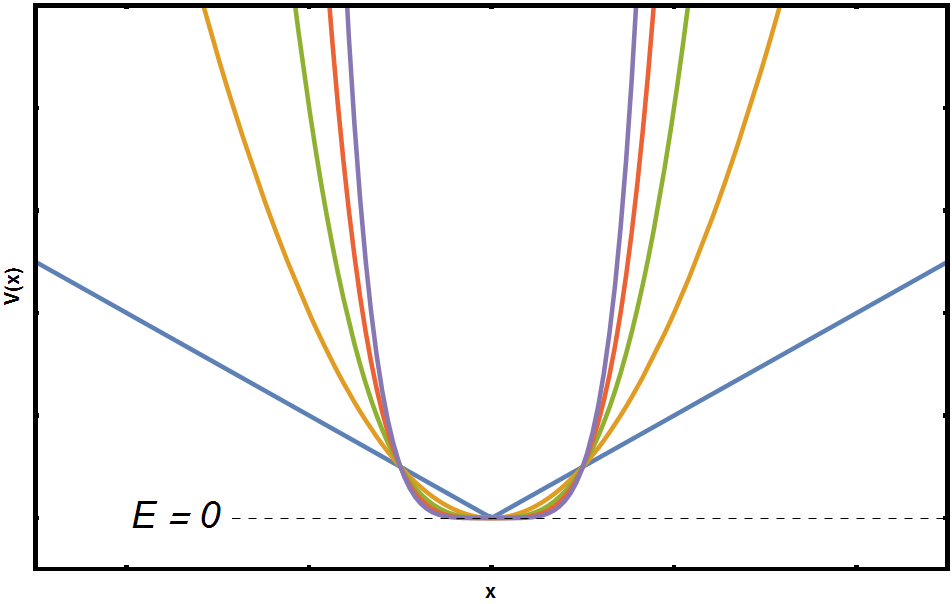
\includegraphics[width=0.8\textwidth,keepaspectratio]{Images/Problem2a.png}
\caption{Plot of the potential energy $V(x) = A|x|^n$ for $n=1,2,3,...,5$}
\label{Prob2a}
\end{figure}
For this given potential we can calculate the period of oscillations for the case where 
$n=2$ by first solving the \emph{Integral of Motion}
\begin{equation}
dt = \int\frac{dx}{\sqrt{2/m(E-V(x))}}.
\label{EQofMot}
\end{equation}
Therefore for $Ax^2$ we see equation \ref{EQofMot} becomes
\begin{align*}
dt &= \int\frac{dx}{\sqrt{2/m(E-Ax^2)}}\\
&\Downarrow\\
dt &= \int\frac{dx}{\sqrt{2A/m(E/A-x^2)}}
\end{align*}
Which we need to integrate from the turning points given by
\begin{align*}
E &= V(x) = Ax^2\\
&\Downarrow\\
x_{\pm} &= \pm\sqrt{\frac{E}{A}}
\end{align*}
to find the total period by
$$T = 2\int_{x_-}^{x_+}\frac{dx}{\sqrt{2A/m(E/A-x^2)}}.$$
This allows us to use a substitution where
$$x = \sqrt{\frac{E}{A}}\sin(\theta)$$
and 
$$dx = \sqrt{\frac{E}{A}}\cos(\theta)d\theta.$$
So, by changing from $x$ to $\theta$ we have
\begin{align*}
T &= 2\int_{x_-}^{x_+}\frac{dx}{\sqrt{2A/m(E/A-x^2)}}\\
&\Downarrow\\
T &= 2\sqrt{\frac{m}{2A}}\int_{x_-(\theta)}^{x_+(\theta)}\frac{\sqrt{E/A}\cos(\theta)d\theta}{\sqrt{(E/A-E/A\sin^2(\theta))}}\\
&= 2\sqrt{\frac{m}{2A}}\int_{x_-(\theta)}^{x_+(\theta)}\frac{\cancel{\sqrt{E/A}\cos(\theta)}d\theta}{\cancel{\sqrt{E/A}\cos(\theta)}}\\
&= 2\sqrt{\frac{m}{2A}}\int_{x_-(\theta)}^{x_+(\theta)} d\theta\\
&\Downarrow\\
T &= \left.2\sqrt{\frac{m}{2A}}\theta\right|_{x_-(\theta)}^{x_+(\theta)}\\
&\Downarrow\\
T &= \left.2\sqrt{\frac{m}{2A}}\arcsin\left(\frac{x}{\sqrt{E/A}}\right)\right|_{x_-}^{x_+}\\
&= 2\sqrt{\frac{m}{2A}}\left(\arcsin\left(\frac{\sqrt{E/A}}{\sqrt{E/A}}\right) - \arcsin\left(\frac{-\sqrt{E/A}}{\sqrt{E/A}}\right)\right)\\
&= 2\sqrt{\frac{m}{2A}}\left(\arcsin\left(1\right) - \arcsin\left(-1\right)\right)\\
&= 2\sqrt{\frac{m}{2A}}\left(\frac{\pi}{2} - \left(-\frac{\pi}{2}\right)\right)\\
&= 2\sqrt{\frac{m}{2A}}\left(\frac{\pi}{2} + \frac{\pi}{2}\right)\\
T &= 2\sqrt{\frac{m}{2A}}\pi
\end{align*}
Note that the period of oscillation does not depend on the energy of the system $E$ this is 
expected for a harmonic potential.

\item Given the potential energy $V(x) = -\frac{V_0}{\cosh^2(\alpha x)}$ where $V_0$ and 
$\alpha$ are positive constants. We plotted this potential in Figure \ref{Prob2b}. Note 
the two dotted lines at $E=-V_0$ and $E=0$ these points define the range of energies that
allow for bounded motion given by
$$-V_0<E<0.$$
\begin{figure}
\centering
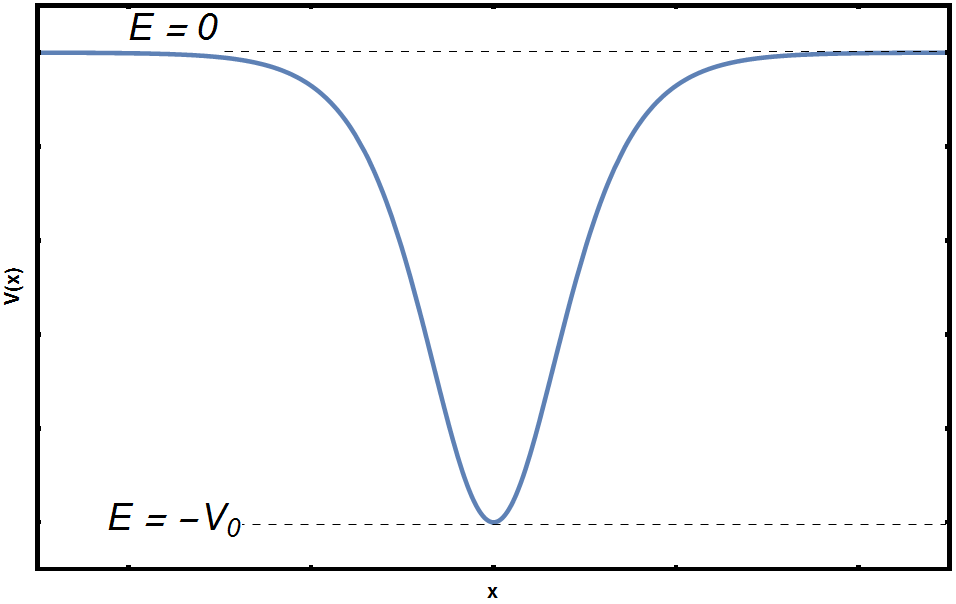
\includegraphics[width=0.8\textwidth,keepaspectratio]{Images/Problem2b.png}
\caption{Plot of the potential energy $V(x) = -V_0\cosh^2(\alpha x)$}
\label{Prob2b}
\end{figure}
For this potential we can calculate the period of oscillations by first solving equation 
\ref{EQofMot} by
\begin{align*}
dt &= \int\frac{dx}{\sqrt{2/m(E-V(x))}}\\
&\Downarrow\\
dt &= \int\frac{dx}{\sqrt{2/m(E+V_0/\cosh^2(\alpha x))}}
\end{align*}
over the bounds given by the turning points found by
\begin{align*}
E &= V(x) = -\frac{V_0}{\cosh^2(\alpha x)}\\
&\Downarrow\\
x_{\pm} &= \pm\frac{\cosh^{-1}\left(\sqrt{\frac{V_0}{E}}\right)}{\alpha}
\end{align*}
Now equation \ref{EQofMot} becomes a definite integral which allows us to find the period of
oscillations by
\begin{align*}
dt &= \int\frac{dx}{\sqrt{2/m(E+V_0/\cosh^2(\alpha x))}}\\
&\Downarrow\\
T &= 2\int_{x_-}^{x_+}\frac{dx}{\sqrt{2/m(E+V_0/\cosh^2(\alpha x))}}\\
&= 2\int_{x_-}^{x_+}\frac{\cosh(\alpha x)dx}{\sqrt{2/m(E\cosh^2(\alpha x)+V_0)}}
\end{align*}
We note that $\cosh^2(\alpha x) = 1 + \sinh^2(\alpha x)$ so that
\begin{align*}
&\Rightarrow 2\int_{x_-}^{x_+}\frac{\cosh(\alpha x)dx}{\sqrt{2/m(E(1+\sinh^2(\alpha x))+V_0)}}\\
&= 2\int_{x_-}^{x_+}\frac{\cosh(\alpha x)dx}{\sqrt{2E/m(1+V_0/E+\sinh^2(\alpha x)}}
\end{align*}
Now we let $a = \sqrt{1+V_0/E}$ and $t = \sinh(\alpha x)$ where
$$dt = \alpha\cosh(\alpha x) dx$$
which transforms our integral into
\begin{align*}
&\Rightarrow\frac{2}{\alpha}\sqrt{\frac{m}{2E}}\int_{t(x_-)}^{t(x_+)}\frac{dt}{\sqrt{a^2+t^2}}
\end{align*}
Next we follow another substitution such that
$$t = a\sinh(u)$$
and
$$dt = a\cosh(u)du$$
so the integral becomes
\begin{align*}
&\Rightarrow\frac{2}{\alpha}\sqrt{\frac{m}{2E}}\int_{u(t(x_-))}^{u(t(x_+))}\frac{a\cosh(u)du}{\sqrt{a^2+a^2\sinh(u)^2}}\\
&= \frac{2}{\alpha}\sqrt{\frac{m}{2E}}\int_{u(t(x_-))}^{u(t(x_+))}\frac{a\cosh(u)du}{\sqrt{a^2\cosh^2(u)}}\\
&= \frac{2}{\alpha}\sqrt{\frac{m}{2E}}\int_{u(t(x_-))}^{u(t(x_+))}\frac{a\cosh(u)du}{a\cosh(u)}\\
&= \frac{2}{\alpha}\sqrt{\frac{m}{2E}}\int_{u(t(x_-))}^{u(t(x_+))}du\\
&= \left.\frac{2}{\alpha}\sqrt{\frac{m}{2E}}u\right|_{u(t(x_-))}^{u(t(x_+))}\\
&\Downarrow\\
&= \left.\frac{2}{\alpha}\sqrt{\frac{m}{2E}}\sinh^{-1}(t/a)\right|_{t(x_-)}^{t(x_+)}\\
&\Downarrow\\
&= \left.\frac{4}{\alpha}\sqrt{\frac{m}{2E}}\sinh^{-1}\left(\frac{\sinh(\alpha x)}{\sqrt{1+V_0/E}}\right)\right|_{0}^{x_+}
\end{align*}
Note due to the symmetry of the potential we changed the bounds of integration from 
$x_-\rightarrow x_+$ to $0\rightarrow x_+$ and doubled the integral without changing the
calculation. Now we note that
\begin{align*}
\sinh(\alpha x_+) &= \sinh\left(\alpha\frac{\cosh^{-1}\left(\sqrt{\frac{V_0}{E}}\right)}{\alpha}\right)\\
&= \sinh\left(\cosh^{-1}\left(\sqrt{V_0/E}\right)\right)\\
&= \sqrt{\frac{V_0}{E}-1}
\end{align*}
Which if we replace into our expression for the period we find
\begin{align*}
T &= \frac{4}{\alpha}\sqrt{\frac{m}{2E}}\sinh^{-1}\left(\frac{\sinh(\alpha x_+)}{\sqrt{1+V_0/E}}\right) - \cancelto{0}{\frac{4}{\alpha}\sqrt{\frac{m}{2E}}\sinh^{-1}\left(\frac{\sinh(0)}{\sqrt{1+V_0/E}}\right)}\\
&= \frac{4}{\alpha}\sqrt{\frac{m}{2E}}\sinh^{-1}\left(\frac{\sqrt{V_0/E-1}}{\sqrt{1+V_0/E}}\right)\\
&= \frac{4}{\alpha}\sqrt{\frac{m}{2E}}\sinh^{-1}\left(\sqrt{\frac{V_0/E-1}{V_0/E+1}}\right)
\end{align*}

\item Given the potential energy $V(x) = V_0\tan^2(\alpha x)$ where $V_0$ is a positive 
constant. This potential is shown in Figure \ref{Prob2c}.
\begin{figure}
\centering
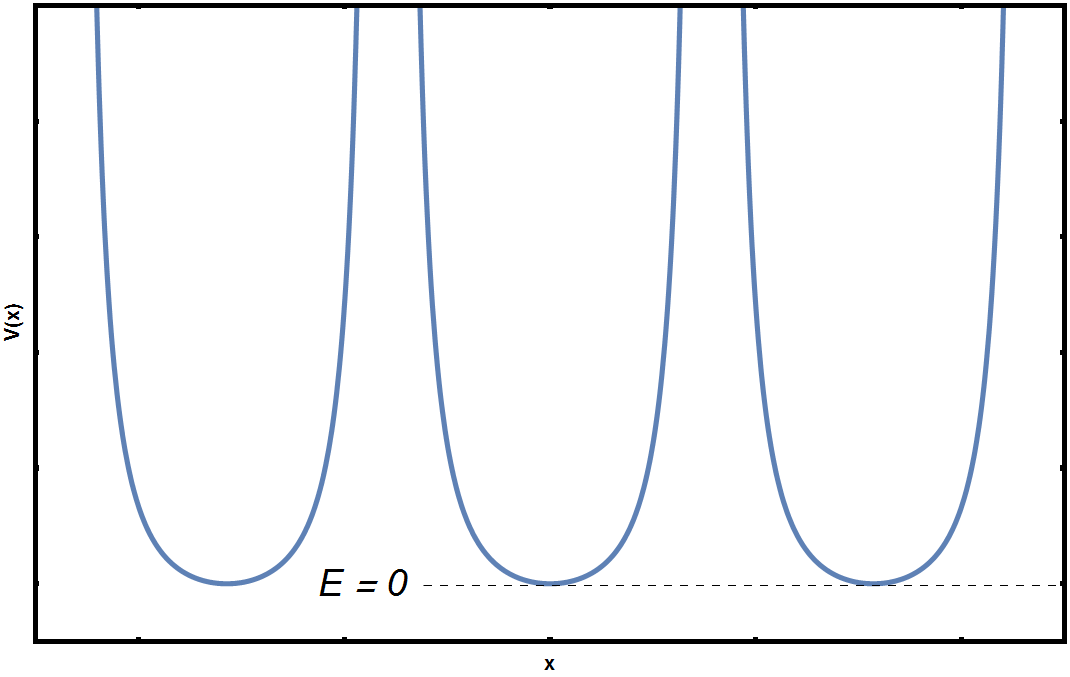
\includegraphics[width=0.8\textwidth,keepaspectratio]{Images/Problem2c.png}
\caption{Plot of the potential energy $V(x) = V_0\tan^2(\alpha x)$}
\label{Prob2c}
\end{figure}
Note that in the range
$$0<E<\infty$$
we have bounded oscillatory motion. Now we can use equation \ref{EQofMot} with the turning
points given by 
\begin{align*}
E &= V_0\tan^2(\alpha x)\\
&\Downarrow\\
x_{\pm} &= \pm \frac{\arctan\left(\sqrt{E/V_0}\right)}{\alpha}
\end{align*}
\end{enumerate}
we can now integrate equation \ref{EQofMot} over $x_{\pm}$ to find the period.
\begin{align*}
T &= 2\int_{x_-}^{x_+}\frac{dx}{\sqrt{2/m(E-V_0\tan^2(\alpha x))}}
&\Downarrow\\
T &= 4\sqrt{\frac{m}{2E}}\int_{0}^{x_+}\frac{dx}{\sqrt{1-V_0/E\tan^2(\alpha x)}}
\end{align*}
Using \emph{Mathematica} we evaluate this integral as
\begin{align*}
T &= 4\sqrt{\frac{m}{2E}}\left.\frac{\arctan\left(\frac{\sqrt{2(1+V_0/E)}\sin(\alpha x)}{\sqrt{1-V_0/E+(1+V_0/E)\cos(2\alpha x)}}\right)\sqrt{1-V_0/E+(1+V_0/E)\cos(2\alpha x)}\sec(\alpha x)}{\sqrt{2(1+V_0/E)(1-V_0/E\tan^2(\alpha x))}}\right|_{0}^{x_+}\\
&= 4\sqrt{\frac{m}{2E}}\frac{\arctan\left(\frac{\sqrt{2(1+V_0/E)}\sin(\alpha x_+)}{\sqrt{1-V_0/E+(1+V_0/E)\cos(2\alpha x_+)}}\right)\sqrt{1-V_0/E+(1+V_0/E)\cos(2\alpha x_+)}\sec(\alpha x_+)}{\sqrt{2(1+V_0/E)(1-V_0/E\tan^2(\alpha x_+))}}\\
\end{align*}

\pagebreak

\section{Problem \#3}
\begin{enumerate}[(a)]
\item For the central force field given by the \emph{Yukawa-potential}
\begin{equation}
V(r) = -k\frac{e^{-\alpha r}}{r},
\label{Yukawa}
\end{equation}
where $k$ and $\alpha$ are positive constants. Note that this potential can be reduced to a
one-dimensional potential using an effective potential given by
\begin{equation}
V_{eff}(r) = V(r) + \frac{L^2}{2mr^2}.
\label{EffPot}
\end{equation}
Note that $L$ is the conserved quantity related to conservation of angular momentum. So we 
can combine equations \ref{Yukawa} and \ref{EffPot} to find the effective potential for this
system as
$$V_{eff}(r) = -k\frac{e^{-\alpha r}}{r} + \frac{L^2}{2mr^2}.$$
\begin{figure}
\centering
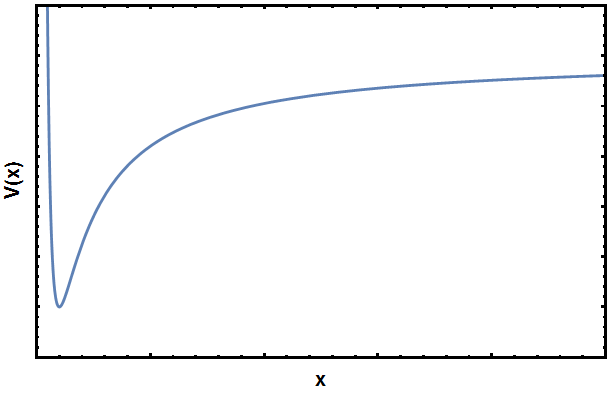
\includegraphics[width=0.8\textwidth,keepaspectratio]{Images/Problem3a.png}
\caption{Plot of the effective potential for the \emph{Yukawa-potential}.}
\label{Prob3a}
\end{figure}
which we plot in Figure \ref{Prob3a}. We can rearrange the effective potential in such a way
to illustrate the effect of angular momentum
$$V_{eff}(r) = A\left(\frac{1}{r^2} - \frac{2km}{L^2}\frac{e^{-\alpha r}}{r}\right)$$
we see that for large $L$ the $r^{-2}$ term dominates and we have a positive energy. This 
corresponds to an unbound orbit. For small $L$ we have energies that are negative. This 
implies that for these $L$ there exists bound orbits with two turning points.

\item When we compare the potential given by equation \ref{Yukawa} we see that it is like a
inverse square law potential given by
$$V(r) = -k\frac{1}{r}$$
the notable difference being the factor of $e^{-\alpha r}$. This factor makes the potential
become smaller faster as $r$ increases. This implies that a $1/r$ potential would have a 
further reach as compared to the \emph{Yukawa-potential}. This implies that there exists 
bound orbits with a greater $r_{max}$.

\item We see that in Figure \ref{Prob3a} that $V_{eff}(r)$ has a minimum. This implies that 
there exists a ground state or circular orbit. We note that this occurs at $r_0$ defined by
\begin{equation}
\frac{dV_{eff}(r_0)}{dr} = 0.
\label{CircOrb}
\end{equation}
Where we first need to change variables such that $r\rightarrow1/u$ which makes our 
effective potential become
\begin{align*}
V_{eff}(r) &= V_{eff}(1/u)\\
&= -k\frac{e^{-\alpha/u }}{1/u} + \frac{L^2}{2m(1/u)^2}\\
&= -kue^{-\alpha/u}+ \frac{L^2}{2m}u^2
\end{align*}
Therefore we can solve for the radius of the ground state in terms of $u$ by
\begin{align*}
\left.\frac{dV_{eff}(u)}{du}\right|_{u_0} &= 0\\
&\Downarrow\\
0 &= \frac{d}{du}\left(-kue^{-\alpha/u} + \frac{L^2}{2m}u^2\right)\\
&= -ke^{-\alpha/u} -kue^{-\alpha/u}\left(\alpha u^{-2}\right) + \frac{L^2}{m}u\\
&= -ke^{-\alpha/u} -k\alpha e^{-\alpha/u}\frac{1}{u} + \frac{L^2}{m}u\\
&= -ke^{-\alpha/u}\left(1 + \alpha\frac{1}{u}\right) + \frac{L^2}{m}u\\
&\Downarrow\\
\frac{L^2}{km} &= r_0\left(1 + \alpha r_0\right)e^{-\alpha r_0}
\end{align*}
Note we can not solve this equation explicitly. So we look at the function
$$f(r_0) =  r_0\left(1 + \alpha r_0\right)e^{-\alpha r_0}$$
and note that the maximum of $f(r_0)$ is found by
\begin{align*}
f'(r_0) = 0 &=  \frac{d}{dr_0}\left(\frac{}{}\left(r_0 + \alpha r_0^2\right)e^{-\alpha r_0}\right)\\
&=  -\left(r_0 + \alpha r_0^2\right)\alpha e^{-\alpha r_0} + \left(1 + 2\alpha r_0\right)e^{-\alpha r_0}\\
&\Downarrow\\
\alpha(r_0 + \alpha r_0^2) &= 1 + 2\alpha r_0\\
(\alpha r_0)^2 - \alpha r_0 &= 1\\
&\Downarrow\\
r^{max}_0 &= \frac{-1\pm\sqrt{5}}{2\alpha}
\end{align*}
Therefore this constrains our angular momentum by the inequality
$$\frac{L^2}{km} < f(r^{max}_0).$$
Where we can solve
\begin{align*}
f(r^{max}_0) &= r^{max}_0\left(1 + \alpha r^{max}_0\right)e^{-\alpha r^{max}_0}\\
&= \left(\frac{-1+\sqrt{5}}{2\alpha}\right)\left(1 + \alpha\frac{-1+\sqrt{5}}{2\alpha}\right)e^{-\alpha (-1+\sqrt{5})/2\alpha}\\
&= \frac{1}{\alpha}\left(\frac{-1+\sqrt{5}}{2}\right)\left(\frac{1+\sqrt{5}}{2}\right)e^{(1-\sqrt{5})/2)}\\
&= \frac{1}{\alpha}2e^{1-\sqrt{5}/2)}
\end{align*}
Which implies that
$$\frac{\alpha L^2}{km} < 2e^{(1-\sqrt{5})/2}$$
Therefore, for large $L$ we see that we have no possible circular orbits.

\item If we add a small perturbation to the ground state orbit which we will call $\Delta r$
we can find the small oscillations about the circular orbit. Doing this we can expand 
$V_{eff}(r)$ about $r_0$ to get
$$V_{eff}(r) = V_eff(r_0) +\cancelto{0}{\Delta r \frac{dV_{eff}(r)}{dr}} + \frac{1}{2}(\Delta r)^2\frac{d^2V_{eff}(r_0)}{dr^2}$$
we note that $V_eff(r_0)$ is an additive constant and due to the fact that potentials are 
relative it can be ignored. Also we define the constant
$$K \equiv \frac{d^2V_{eff}(r_0)}{dr^2}$$
so we can say our equation of motion for the perturbed state is
$$V_{eff}(\Delta r) = m\ddot{\Delta r} = -K\Delta r.$$
Note that this produces a solution of the form 
$$\Delta r = A\cos(\omega_r t)$$
where
$$\omega_r = \sqrt{\frac{K}{m}}$$
so we can see that the period of oscillation is given by $\omega_r$ by
$$T = \frac{2\pi}{\omega_r} = 2\pi\sqrt{\frac{m}{K}}$$
so to find the period of oscillation around the circular orbit we need to find $k$. Note 
that we use the variable $u$ as before
\begin{align*}
\left.\frac{d^2V_{eff}(u)}{du^2}\right|_{u_0} &= \frac{d}{du}\left(-ke^{-\alpha/u}\left(1 + \frac{\alpha}{u}\right) + \frac{L^2}{m}u\right)\\
&= -k(\alpha u^{-2})e^{-\alpha/u}\left(1 + \frac{\alpha}{u}\right) - ke^{-\alpha/u}\left(-\alpha\frac{1}{u^2}\right) + \frac{L^2}{m}\\
&= -k(\alpha u^{-2})e^{-\alpha/u}\left(1 + \frac{\alpha}{u}\right) + k\alpha e^{\alpha/u}\left(\frac{1}{u^2}\right) + \frac{L^2}{m}\\
&= -k\alpha e^{-\alpha/u}\left(\frac{1}{u^2} + \frac{\alpha}{u^3} - \frac{1}{u^2}\right) + \frac{L^2}{m}\\
&= -k\alpha^2e^{-\alpha/u}\frac{1}{u^3} + \frac{L^2}{m}\\
&\Downarrow\\
&= -k\alpha^2e^{-\alpha r_0}r_0^3 + \frac{L^2}{m}\\
\end{align*}
Note that from part (c) we found that for circular orbits 
$$\frac{L^2}{m} = -ke^{-\alpha r}(1+\alpha r)r$$
so we can say that 
$$K = -ke^{-\alpha r_0}(\alpha^2r_0^3 + \alpha r_0^2 + r_0)$$
\end{enumerate}
so the period of small oscillations is given by
$$T = 2\pi\sqrt{\frac{m}{-ke^{-\alpha r_0}(\alpha^2r_0^3 + \alpha r_0^2 + r_0)}}$$

\pagebreak

\section{Problem \#4}
\begin{enumerate}[(a)]
\item Given a central force potential 
$$V(r) = \alpha \log(r)$$
we can write the effective potential by equation \ref{EffPot} so that
$$V_{eff}(r) = \alpha\log(r) + \frac{L^2}{2mr^2}$$
Recall for circular orbits we know that
\begin{align*}
\left.\frac{dV_{eff}(r)}{dr}\right|_{r_0} &= 0\\
&\Downarrow\\
0 &= \frac{d}{dr}\left(\alpha\log(r) + \frac{L^2}{2mr^2}\right)\\
0 &= \alpha\frac{1}{r_0} - \frac{L^2}{mr_0^3}\\
&\Downarrow\\
\alpha\frac{1}{r_0} &=  \frac{L^2}{mr_0^3}\\
&\Downarrow\\
\alpha\frac{r_0^3}{r_0} &=  \frac{L^2}{m}\\
&\Downarrow\\
r_0 &=  \frac{L}{\sqrt{m\alpha}}
\end{align*}

\item We can test if the circular orbit in part (a) is stable by
$$\frac{d^2V_{eff}(r_0)}{dr^2} > 0$$
So we can calculate
\begin{align*}
\frac{d^2V_{eff}(r)}{dr^2} &= \frac{d}{dr}\left(\alpha\frac{1}{r}-\frac{L^2}{mr^3}\right)\\
&= -\alpha\frac{1}{r^2}+\frac{3L^2}{mr^4}
\end{align*}
And now we can replace 
$$r= r_0 = \frac{L}{\sqrt{2m\alpha}}$$
such that
\begin{align*}
\frac{d^2V_{eff}(r_0)}{dr^2} &= -\alpha\frac{1}{r_0^2}+\frac{3L^2}{mr_0^4}\\
&= -\alpha\frac{m\alpha}{L^2}+\frac{3L^2}{m}\frac{(m\alpha)^2}{L^4}\\
&= -\frac{m\alpha^2}{L^2}+\frac{3m\alpha^2}{L^2}\\
&= \frac{2m\alpha^2}{L^2}
\end{align*}
Note that by definition $\alpha$, $m$, and $L$ are positive constants therefore
$$\frac{d^2V_{eff}(r_0)}{dr^2} > 0.$$
Which implies that the circular orbit at $r=r_0$ is stable.

\item We can find the frequency of small oscillations about the circular orbit by
$$\Delta r = A\cos(\omega_r t)$$
where
$$\omega_r = \sqrt{\frac{k}{m}}$$
and
$$k \equiv \frac{d^2V_{eff}(r_0)}{dr^2}.$$
Note see the derivation of these equations in problem 3 part (d). Given that 
$$\frac{d^2V_{eff}(r_0)}{dr^2} = \frac{2m\alpha^2}{L^2}$$
we can find $\omega_r$ by
\begin{align*}
\omega_r &= \sqrt{\frac{k}{m}}\\
&= \sqrt{\frac{2m\alpha^2}{mL^2}}\\
&= \sqrt{\frac{2\alpha^2}{L^2}}\\
&= \sqrt{2}\frac{\alpha}{L}
\end{align*}

\item To test if the small oscillations about $r$ given above forms a closed orbit we test
if 
$$\frac{\omega_r}{\omega_{\theta}}\in\mathbb{Q}$$
which states that the ratio between the frequency of small oscillations, $\omega_r$, and the 
orbital frequency, $\omega_{\theta}$, is a rational quotient. Therefore we note that for a
circular orbit there exists a \emph{centripetal force} given by
\begin{equation}
-F_c(r) = \frac{dV(r)}{dr} = m\omega_{\theta}^2 r.
\label{CentFor}
\end{equation}
So, for $V(r) = \alpha\log(r)$ we see that solving equation \ref{CentFor} for 
$\omega_{\theta}$ yields
\begin{align*}
m\omega_{\theta}^2 r &=  \frac{d}{dr}\left(\alpha\log(r)\right)\\
m\omega_{\theta}^2 r &=  \frac{\alpha}{r}\\
&\Downarrow\\
\omega_{\theta}  &=  \sqrt{\frac{\alpha}{mr_0^2}}\\
&=  \sqrt{\frac{\alpha}{m}\frac{m\alpha}{L^2}}\\
&=  \sqrt{\frac{2\alpha^2}{L^2}}\\
&=  \frac{\alpha}{L}
\end{align*}
Note we evaluate equation \ref{CentFor} at the radius of circular orbit, $r_0$. So we can
evaluate
\begin{align*}
\frac{\omega_r}{\omega_{\theta}} &= \frac{\sqrt{2}\cancel{\frac{\alpha}{L}}}{\cancel{\frac{\alpha}{L}}}\\
&= \sqrt{2} \notin \mathbb{Q}
\end{align*}
We see that the ratio is not a rational quotient, therefore the oscillations about the 
circular orbit do not form a closed orbit.
\end{enumerate}
\end{document}

